\chapter{Обзор документации к устройствам}
\label{cha:analysis}

В этой главе будет проведен обзор документации, предоставляемой
к исследуемому wifi-чипу CC3100, отладочной установке CC3100BOOST
и ее связке с CC31XXEMUBOOST.

Важным предварительным моментом является то, где была получена
документация. Конечно, хорошо иметь переведенный и адаптированный
материал на родном, русском, языке, но обычно данные источники
быстро устаревают, после обновления исходной документации на
официальном сайте, а также очень часто могут содержать
ошибки и неточности, возникшие при переводе, либо ошибки,
унаследованные от первоисточников, без учета списка опечаток,
предоставляемых Texas Instruments. Поэтому стоит использовать
документы, распространяемые вместе странице продукта (как на рисунке \ref{cc3100-docs}),
а также использовать Вики-ресурс посвященный линейке CC31XX\cite{cc3100wiki}.

\vspace{2cm}
\myImage{Основные источники информации (Выделено красным)}{cc3100-docs}{cc3100-docs}
\vspace{2cm}
\clearpage

\section{CC3100}

Рассмотрим основные источники информации к главному в нашем
исследовании устройству -- СС3100. В нашем случае,
это два основных технических описания:

\begin{enumerate}
    \item Техническое описание процессора (\textit{Datasheet})\cite{cc3100datasheet};
    \item Руководство пользователя (\textit{User Guide})\cite{cc3100userguide}.
\end{enumerate}

Основные характеристики \textit{CC3100 SimpleLink Wi-Fi}:

\begin{itemize}
    \item Состоит из Интернет процессора и подсистемы управления питанием;
    \item Wi-Fi Интернет подсистема:
        \begin{itemize}[$\star$]
            \item ARM микроконтроллер для полной обработки Интернет-протоколов и
            связи с внешним микроконтроллером;
            \item Поддержка 802.11 b/g/n;
            \item Поддержка WPA2 Personal and Enterprise;
            \item Работа в режиме станции, точки доступа и Wi-Fi ретранслятора;
            \item стек протоколов TCP/IP:
            \begin{itemize}
                \item До 8 одновременных TCP или UDP соединений;
                \item До 2 одновременных TLS и SSL соединений.
            \end{itemize}
            \item Пропускная способность:
            \begin{itemize}
                \item UDP: 16 Мбит/c;
                \item TCP: \textbf{13 Мбит/с}.
            \end{itemize}
        \end{itemize}
    \item Подсистема управления питанием:
    \begin{itemize}[$\star$]
        \item $V_{BAT}$ Wide-Voltage режим: от 2.1 до 3.6 Вольт;
        \item Предустановленный $1.85$-Вольт режим.
    \end{itemize}
\end{itemize}

Более подробные характеристики указаны в тех. описании\cite{cc3100datasheet}.
Главным для нашего исследования будет являться проверка заявленной
пропускной способности (выделено жирным).

Хорошей иллюстрацией устройства внутренних подсистем и модулей
изображено в техническом описании на рисунках \ref{cc3100-logic-structure} и
\ref{cc3100-internet-stack}.
\mySecondImage{Основные модули и подсистемы CC3100}{cc3100-logic-structure}{cc3100-logic-structure}{0.5}
\mySecondImage{Стек Интернет протоколов, реализованных в рамках CC3100.
Также есть возможность реализации своих протоколов на внешнем микроконтроллере}{cc3100-internet-stack}{cc3100-internet-stack}{0.5}
\clearpage

Следующим важным моментом, который нужно рассмотреть в устройстве
чипа -- это как производится его управление с помощью внешнего микроконтроллера.
CC3100 поддерживает иммет два типа портов -- \textit{UART} и \textit{SPI}.
Первый, \textit{Universal Asynchronous Receiver-Transmitter}\cite{uart} --
Универсальный асинхронный приёмопередатчик, используется для
перепрошивки и первоначальной настройки чипа. В то время
управление осуществляется через SPI (\textit{Serial Peripheral Interface})\cite{spi}.

Шина SPI рассчитана на несимметричное соединение двух микроконтроллеров -- один
из них, ведущий (\textit{master}), всегда инициирует обмен данными, на что второй,
ведомый (\textit{slave}), принимает данные и может в ответ
передать аналогичное количество байт. В классическом
виде SPI-шина состоит из четырех основных соединений (проводов):
\begin{itemize}
    \item Chip Select или Slave Select /  $\overline{CS}$ или $\overline{SS}$ -- выбор устройства,
    на который будет происходить передача;
    \item Clock / CLK -- тактовый сигнал;
    \item Master Output Slave Input / MOSI -- выходной сигнал ведущего микроконтроллера;
    \item Master Input Slave Output / MISO -- входной сигнал для ведущего микроконтроллера.
\end{itemize}

Передача происходит при установке мастером сигнала $\overline{CS}$,
что сигнализирует выбор нужного устройтва
(Мастер может иметь несолько линей $\overline{CS}$
для соединения с разными устройствами, при этом остальные провода
могут быть подключены к одному и тому же порту). Далее,
в зависимости от двух параметров: начало синхронизации
с верхнего или нижнего уровня CLK и выборка данных происходит
по заднему или переднему фронту CLK, SPI начинает считывать
данные оцифрованные сигналы с шин MOSI и MISO.

На рисунке \ref{cc3100-spi-timing} изображены основные промежутки
времени для работы по SPI.
\clearpage

\myImage{Основные временные характеристики SPI СС3100}{cc3100-spi-timing}{cc3100-spi-timing}
\begin{table}[h]
\caption{Основные характеристики SPI-соединения}
\label{spi:timing}
\begin{center}
    \begin{tabular}{|c|c|}
        \hline
        Номер параметра & Название параметра \\ \hline
        l2 & тактовый период \\ \hline
        l6 & время на установку RX \\ \hline
        l7 & период удерживания RX\\ \hline
        l8 & задержка вывода TX \\ \hline
        l9 & период удерживания TX \\ \hline
    \end{tabular}
\end{center}
\end{table}

Для полноценной работы всего стека Интернет протоколов
чипу СС3100 тербуется внешняя flash-память, соединенная
по SPI, изображенная на схеме \ref{cc3100-spi-flash}.


\mySecondImage{Схема соединения CC3100 с внешней flash-памяти}{cc3100-spi-flash}{cc3100-spi-flash}{0.6}
Для управления внешним микроконтроллером используется более
хитрое, 6-ти проводное, соединение (Рисунок \ref{cc3100-spi-mcu}).
Помимо основных SPI-соединений при управлении требуется еще
$nHIB$ сигнал для выключения wifi-чипа в режим сна (\textit{Hibernate}),
а сигнал INTR (\textit{Interrupt}) потребуется для инициации прерывания со стороны
Wi-Fi.

\mySecondImage{Схема соединения CC3100 с ведущим микроконтроллером}{cc3100-spi-mcu}{cc3100-spi-mcu}{0.6}

Наконец, рассмотрим руководство для разработчика, содержащее
множество примеров и пояснений, как программно работать с
API драйвера, поставляемым вместе с CC3100, а так же кратко
и на примерах объясняющее ту или иную поддерживаемую технологию,
иллюстрируя это примером программы.

На данном этапе полезно ознакомится с описанием базового конечного,
автомата, который необходимо реализовать для полноценного управления
Wi-Fi подсистемой (Рисунок \ref{cc3100-state-machine}).

\myImage{Базовый конечный автомат для работы с Wi-Fi чипом}{cc3100-state-machine}{cc3100-state-machine}

\clearpage

\section{CC3100BOOST \& CC31XXEMUBOOST}

Рассмотрим набор руководств прилагающихся к CC3100BOOST и CC31XXEMUBOOST,
обеспечивающих предворительной установкой для тестирования Wi-fi чипа.
При желании, можно скачать с сайта Texas Instruments более подробное
описание устройства их схем, но для быстрого старта будет достаточно
следующих руководств:

\begin{itemize}
    \item Руководство для быстрого старта (\textit{Getting started guide})\cite{cc3100boostgetstart};
    \item Руководство для пользователя (\textit{User guide})\cite{cc3100boostuserguide}.
\end{itemize}


\begin{figure}[!hbt]
    \begin{subfigure}{0.5\textwidth}
        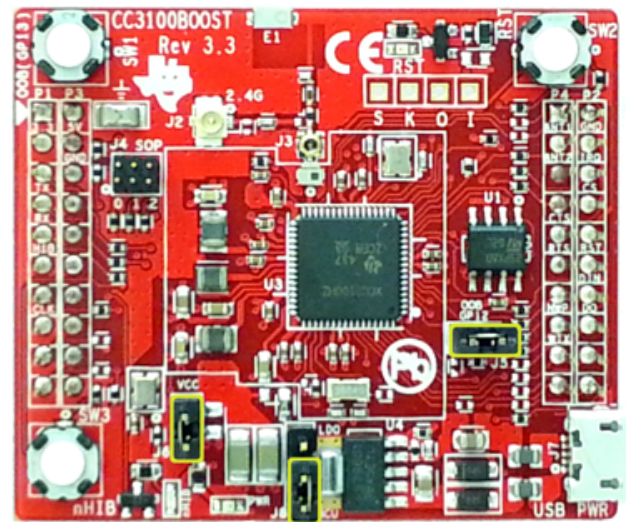
\includegraphics[width=\textwidth]{figures/getstart-boost}
        \caption{CC3100BOOST}
        \label{fig13:a}
    \end{subfigure}
    ~
    \begin{subfigure}{0.5\textwidth}
        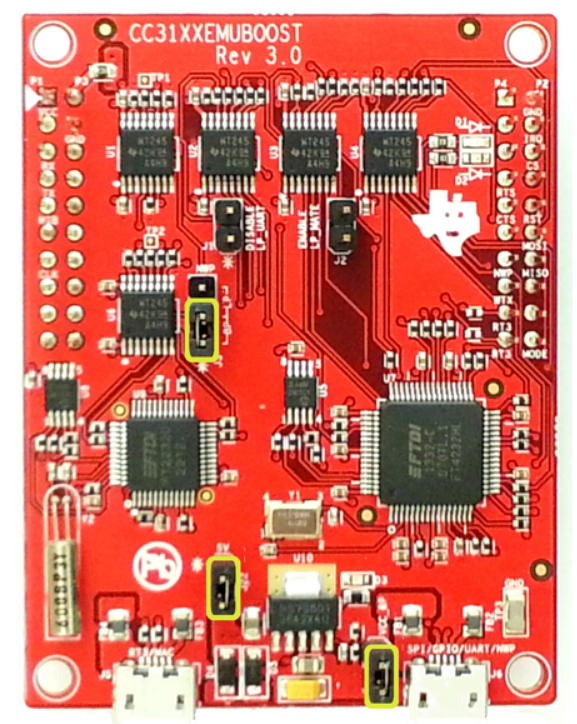
\includegraphics[width=\textwidth]{figures/getstart-emuboost}
        \caption{CC31XXEMUBOOST}
        \label{fig13:b}
    \end{subfigure}

    \caption{Расположение джамперов на CC3100BOOST и CC31XXEMUBOOST для совместной работы}
    \label{fig_13}
\end{figure}

В руководстве для быстрого старта можно найти краткое описание
устройств, а также процесс сборки, как самих схем, так и распаковки
SDK и настройки сред разработки для запуска первых программ.
На рисунке \ref{fig_13} выделено необходимое расположение
джамперов (переключателей) для совместной работы. После их
установки остается соединить обе платы между собой, чтобы
совпали белые треугольники отмаркированные на плате.
Фото данных плат в другом ракурсе и получившуюся конструкцию
можно рассмотреть в Приложении \ref{cha:appendix1}.

В руководстве же пользователя, можно найти более детальное
описание схемы CC3100BOOST, ка например расположение основных
элементов на схеме (Рисунок \ref{boost-logic-scheme}) от
расположения внешней антены до элементов питания, а также способах измерения входного
напряжения.
\vspace{4cm}
\mySecondImage{Рассположение элементов на CC3100BOOST}{boost-logic-scheme}{boost-logic-scheme}{0.8}

\clearpage

\myImage{Вывод ножек CC3100 на плате BOOST}{boost-pins}{boost-pins}
\vspace{3cm}

Также, одним из самых интересных описаний в этой схеме,
является вывод ножек на внешние выводы (Рисунок \ref{boost-pins}).
Так, рассмотрев в предыдущем разделе выводы самого CC3100
мы видим необходимые нам SPI\_CS, SPI\_CLK, SPI\_MOSI, SPI\_MISO
для соединения с внешним микроконтроллером по SPI, а также
сигналы nHIB и IRQ для лучшего управления чипом.
В добавок к этому, для полноценной проверки прототипа
будующего устройства мы можем подвести внутреннее питание
от целевого устройства на ножки VCC или $+5V$, и заземлить
чип на ножках $GND$.


%%% Local Variables:
%%% mode: latex
%%% TeX-master: "rpz"
%%% End:
